\chapter{Použité technologie a teorie}
V této kapitole jsou uvedeny informace týkající se technologií využítých při implementaci hry. Každá z nich je stručně představena a uvedena do souvislosti s touto prací. Mimo těchto informací kapitola také obsahuje teorii nutnou k pochopení postupů použitých při implementaci.

\label{chap:teorie}
\section{HTML5}
\label{section:html5}
HTML5\footnote{\url{http://www.w3.org/TR/html5/}} je připravovaným webovým standardem, který v první řadě vylepšuje podporu zobrazení multimediálního obsahu prostřednictvím webového prohlížeče. Co se týče doby od vydání předchozí specifikace HTML4.01\footnote{\url{http://www.w3.org/TR/REC-html40/}}, je nováčkem na poli webových technologií a jeho finální specifikace není v době psaní této práce stále dokončena. Vzhledem k tomu, že technologie  zahrnuté v jeho specifikaci řeší mnohé praktické problémy, vývojáři webových prohlížečů již nyní jednotlivé prvky HTML5 implementují. Experimenty s prohlížeči tak dávají pracovním skupinám spravujícím tuto specifikaci zpětnou vazbu, na jejímž základě lze provést mnohá vylepšení. Významnou vlastností specifikace je zpětná kompatibilita s její předchozí verzí, což umožňuje zobrazovat nové typy dokumentů v prohlížečích, které tyto technologie doposud neimplementují.~\cite{pilgrim2010html5, macdonald2011html5, lubbers2011pro}

Nejprve bude zmíněn historický vývoj a rozdělení HTML5 technologií, poté bude uveden výčet některých nových syntaktických a sémantických elementů, za nímž bude následovat popis elementu \texttt{<canvas>}, který je použit při implementaci hry.

\subsection*{Historie}
\label{subsection:historieHTML5}
Roku 2004 představili Mozilla Foundation a Opera Sorfware na W3C konzorciu návrh, který odrážel současné požadavky na webové aplikace. Tento návrh se soustředil na technologie, které by byly zpětně kompatibilní s tehdejšími webovými prohlížeči a zahrnoval také počáteční návrh specifikace Web Forms 2.0. Hlasování konzorcia dopadlo v neprospěch návrhu, což vedlo k tomu, že pracovní skupina W3C nadále soustředila své prostředky na vývoj specifikace XHTML2. Požadavky na webové aplikace však zůstaly nevyslyšeny, a tudíž byla hlavními představiteli vývojářů webových prohlížečů vytvořena nová pracovní skupina s názvem Web Hypertext Application Technology Working Group (WHATWG). O pět let později, roku 2009, zanechala W3C snahy protlačit specifikaci XHTML2 a spojila se s pracovní skupinou WHATWG, aby své usilí zaměřily na vývoj společného standardu HTML5.~\cite{pilgrim2010html5, macdonald2011html5, lubbers2011pro}

Značné popularity HTML5 nabylo po roce 2010, kdy tehdejší výkonný ředitel firmy Apple, Steve Jobs, prohlásil~\footnote{\url{https://www.apple.com/hotnews/thoughts-on-flash/}}, že na svých zařízeních nebudou nadále podporovat obsah zobrazovaný pomocí technologie Adobe Flash a zaměří se na podporu HTML5. Vzhledem k zastoupení této firmy na trhu začala valná většina velkých webových společností svůj obsah nabízet i pomocí této technologie.

V březnu roku 2011 vytyčila W3C cíle pro vývoj HTML5, kde určila rok 2014 jako cílový pro přijetí specifikace. Podmínky tohoto přijetí jsou 2 plně funkční implementace. Již dnes jsou mnohé implementace prvků stabilní a připraveny k použití. Jednou z nich je právě v implementaci hry využitý element \texttt{<canvas>}.


\subsection*{Rozdělení HTML5 technologií}
\label{subsection:rozdeleniHTML5}
Diagram technologií a jejich rozdělení je vyčleněn do přílohy~\ref{priloha:html5}. V následujících odstavcích jsou tyto kategorie stručně popsány. \\

\textbf{Oficiální W3C specifikace} zahrnuje nové syntaktické a sémantické elementy, nové a vylepšené web widgety, podporu pro audio/video a také element \texttt{<canvas>}, který slouží k vykreslování grafiky pomocí JavaScriptu. Tato část zahrnuje většinu prvků HTML5, které jsou prohlížeči dobře podporovány. 

\textbf{Prvky původního návrhu} patřily do specifikace, kterou připravila pracovní skupina WHATWG. Většina z nich vyžaduje ke své práci JavaScript a mezi ty nejdůležitější patří \textit{Local Data Storage} a \textit{Offline aplikace}. 

\textbf{Prky, které jsou často zahrnovány do HTML5} jsou například CSS3 a nástroje pro geolokaci.



\subsection*{Nové syntaktické a sémantické elementy HTML5}
\label{subsection:newElementsHTML5}
Nové sémantické elementy rozšiřují možnosti rozlišení úseků značkovaného textu. Na místě, kde byla typicky použita značka \texttt{<div>}, nebo \texttt{<span>} je nyní možné použít značky jako \texttt{<nav>} pro navigaci webu a dále pak například element \texttt{<footer>}, který označuje patičku dokumentu. 

\textbf{Video} a \textbf{audio} data byla v předchozích verzích HTML vkládána do dokumentů pomocí elementu \texttt{<object>}. Ten umožňoval označit obsah interpretovaný zásuvným modulem prohlížeče, kterým byl pro přehrávání videa nejčastěji Adobe Flash. Ten však díky novým možnostem HTML5 a přístupu firem jako Apple postupně ztrácí své dominantní postavení.

\pagebreak

\subsection*{Technologie HTML5 použité při implementaci}
\label{subsection:html5aImplementace}
Použité technologie:

\begin{itemize}
\item Canvas API\footnote{V textu lze často nalézt pojem API. API, neboli Applicaton Programming Interface je, jak z názvu vyplývá, rozhraní pro programování aplikací. Jedná se o sbírku procedur, funkcí, či tříd, které může programátor při tvorbě aplikace využívat.} 
\item WebGL
\item DOM API (Součást HTML5 Microdata)
\item Web Audio API
\end{itemize}

Z technologií HTML5 je při implementaci hry primárně využito \textbf{Canvas API}, které umožňuje prostřednictvím \textbf{WebGL} (podkapitola~\ref{section:webgl}) přistupovat k elementu \texttt{<canvas>} a vykreslovat tak 3D grafiku. \textbf{DOM API} je rozhraní pro přístup k prvkům zobrazovaného dokumentu a slouží k modifikaci jejich obsahu, struktury, nebo stylu, kterým jsou zobrazovány. \textbf{Web Audio API} je rozhraním elementu \texttt{<audio>}, které slouží k přehrávání herní hudby. Původní návrh hry zahrnoval také využítí technologie \textbf{localStorage}, která umožňuje uchovávat herní data na straně klienta bez nutnosti jejich načítaní při obnovení webové stránky. Vzhledem k tomu, že dnešní prohlížeče mají omezení na množství uložených dat\footnote{\url{http://dev-test.nemikor.com/web-storage/support-test/}}, nenalézá tato technologie v implementaci smysluplné využití. Na diagramu~\ref{priloha:html5} je také vyznačen JavaScriptový framework \textbf{jQuery}, jehož je využito hlavně pro vytvoření různých animací webu.

\subsection*{HTML5 \texttt{<canvas>}}
\label{subsection:HTML5canvas}
Základní HTML5 Canvas API obsahuje \textbf{2D} kontext, který umožňuje vykreslovat různé typy tvarů, text a také umožňuje zobrazovat obrazová data přímo do oblasti elementu \texttt{<canvas>}. Pro vykreslování je možné volit různé barvy, rotovat s prvky, zprůhledňovat je, či manipulovat s jednotlivými pixely tohoto elementu.

V souvislosti s WebGL mluvíme o \textbf{3D} kontextu, který umožňuje přímé vykreslování bitmapy, jejíž obsah je možné měnit pomocí JavaScriptu. U 3D kontextu je při každém volání vykreslovacího rozhraní plocha elementu zcela překreslena a je tedy programátorovou prací připravit vykreslovaný obraz před každým voláním. Tím se \texttt{<canvas>} odlišuje od technologií jako Flash, Silverlight, nebo SVG, které vykreslovaný obraz pouze aktualizují (umožňují například posouvat vykreslované objekty scény vůči své aktuální pozici), což na jednu stranu programátora odstiňuje od nízkoúrovňových operací, avšak na stranu druhou má programátor omezenou kontrolu nad výsledným vykresleným obrazem. Podrobnější informace o tom, jak vykreslování pracuje jsou součástí podkapitoly~\ref{section:webgl}.

\pagebreak

\section{Javascript}
\label{section:javascript}
Většina webových stránek se dnes podobá plnohodnotným desktopovým aplikacím právě díky JavaScriptu. JavaScript je programovací jazyk, který umožňuje vylepšit zobrazovaný dokument prostřednictvím animací, interaktivitou, nebo dynamickými visuálními efekty. Jeho velkou výhodou je to, že stránky reagují na podněty uživatele okamžitě - při vyplňování formuláře, nebo v moment, kdy uživatel pohne myší na určitou pozici. Jeho zpracování je totiž oproti jiným skriptovacím jazykům používaným na webu prováděno na klientském zařízení (avšak nejen tam, jak bude uvedeno dále). V současné době je jeho masivní využití vidět v projektech jako Facebook\footnote{\url{www.facebook.com}}, nebo například Google Maps\footnote{\url{maps.google.com}}.

Popularita tohoto jazyka roste a s ním i jeho využití. Nejen, že jeho interprety lze dnes nalézt ve všech webových prohlížečích na stolních počítačích, herních konzolích, chytrých telefonech či tabletech, ale je využit také pro popis grafických rozhraní desktopových aplikací, nebo jako jazyk použitý na straně serveru. Příklady využití JavaScriptu mimo web jsou uvedeny v následujícím přehledu.

\begin{itemize}
\item Doplňky pro prohlížeč Google Chrome, Opera, Safari
\item Apple dashboard widgety
\item JavaScript v pdf souborech
\item Skriptování v Adobe Photoshop, Illustrator, InDesign
\item Zpracování signálu v Max/MSP pro program Ableton Live
\item Skriptování v Unity
\item JavaScript v prostředí Javy
\item Popis grafického rozhraní v knihovně Qt
\item \ldots
\end{itemize}

\subsection*{Historie jazyka}
\label{subsection:jsHistorie}
Autorem jazyka je Brendan Eich z tehdejší společnosti Netscape. Jazyk byl nejdříve vyvíjen pod názvem \textit{\uv{Mocha, LiveScript}}, avšak s vydáním prohlížeče Netscape 2.0B3, jehož byl tento jazyk součástí, se název z marketingových důvodů změnil na JavaScript. Jeho velký úspěch vedl k tomu, že společnost Microsoft vytvořila jeho obdobu pro svůj prohlížeč Internet Explorer, kterou nazvala JScript. V roce 1997 byl jazyk standardizován pod názvem ECMAScript, ze kterého byly následně odvozeny i další implementace, jako je například ActionScript. Svého největšího rozmachu se tento jazyk dočkal s rozšířením technik, které se souhrnně označují jako AJAX (\ref{subsection:AJAX}).\cite{flanagan2006javascript}

\subsection*{Stručný popis jazyka JavaScript}
\label{subsection:jsPopis}
JavaScript je multiplatformní, dynamický, slabě typovaný skriptovací jazyk. Podporuje různá paradigmata včetně objektového, čehož je v implementaci hry často využíváno. Syntaxe jazyka je ovlivněna konvencemi jazyků Java a C, principiálně je však jazyk vystavěn podobně jako jazyky Self a Scheme. Způsob, jakým jsou vytvářeny objekty, je zde oproti klasickým jazykům jako C++ nebo Java odlišný díky tomu, že je tento jazyk prototypově založený. Třídy jsou tak nahrazeny konstruktory objektů a dědičnost prototypováním.\cite{flanagan2006javascript} Příklad vytvoření konstruktoru objektu a jeho následné použití je uveden ve zdrojovém kódu~\ref{code:jsObjectConstructor}.
%\medskip
\begin{lstlisting}[caption=Příklad vytvoření objektu v JavaScriptu,label=code:jsObjectConstructor]
function TestObject(num){

    this.property1 = 1;
    this.property2 = this.property1;
    this.property3 = num;
}

var test = new TestObject(5);
alert(test.property1); // 1
alert(test.property2); // 1
alert(test.property3); // 5

test.property1 = 6;
alert(test.property1); // 6
\end{lstlisting}

JavaScript interaguje s webovou stránkou prostřednictvím dříve popsaného rozhraní DOM tak, že se naváže zpracování událostí vytvářených uživatelem na funkce, které je zpracovávají. Rozhraní DOM však není přesně standardizované a prohlížeče ho implementují různě. U některých prvků je tedy nutné rozlišovat, který prohlížeč JavaScript aktuálně interpretuje a dle toho volit, jakým způsobem se s nimi bude nakládat. Jako příklad je ve zdrojovém kódu~\ref{code:jsMouseEvent} uvedeno zpracování události pohybu kolečka myši.

\begin{lstlisting}[caption=Zpracování události pohybu kolečka myši,label=code:jsMouseEvent]
function handleWheel(event) {
    var delta = 0;
    
    // Zpracování události v Internet Exploreru
    if (!event){
       event = window.event;
    }
	
		// Internet Explorer, Opera, Chrome
		if (event.wheelDelta) {
	    	delta = event.wheelDelta / 120;
		}
		// Mozilla Firefox
		else if (event.detail) {
	    	delta = -event.detail / 3;
		}
    // ...
}
\end{lstlisting}

\subsection*{AJAX}
\label{subsection:AJAX}
AJAX, neboli Asynchronous JavaScript and XML, je souhrnné označení pro vzájemně propojené techniky používané na klientské straně webových aplikací. Tyto techniky umožňují asynchronně nahrát data ze serveru, což pro uživatele znamená, že aktuálně zobrazená webová stránka nemusí být znovu načtena a interakce s aplikací je tak mnohem přívětivější. Využívá se přitom \texttt{XMLHttpRequest} objektu, který je dostupný prostřednictvím JavaScriptu. Navzdory názvu, který vyzdvihuje přenos dat ve formátu XML, je možné použít i formáty jiné. Ve hře je těchto technik využito k načtení herních úrovní, které jsou reprezentovány soubory formátu JSON a následně pak potřebných textur a lightmap. 

%diagram AJAX

\subsection*{JavaScript Frameworky}
\label{subsection:jsFrameworky}
JavaScriptové frameworky slouží k urychlenému vývoji webových aplikací. Vytvářejí jakousi vrstvu nad základními prostředky jazyka a poskytují k nim tak zjednodušený přístup. Frameworků pro jazyk JavaScript existuje celá řada, avšak pro implementaci bylo využito jednoho z nejznámějších - jQuery.

jQuery umožňuje přistupovat k prvkům DOM tak, že se rozdíly mezi prohlížeči (jako třeba právě zpracování události kolečka myši) stírají a k prvkům je tak přistupováno jednotnou formou. Za základě událostí generovaných uživatelem je také umožněno animovat vzhled prvků dokumentu - měnit jejich pozice, průhlednost, či například vrstvu, ve které se mají zobrazit. Toho je ve hře využito velmi často, avšak vzhledem k tomu, že se jedná o animace webu samotného, který není přímou součástí této práce, nebude jejich popisu věnováno mnoho prostoru. Příklad animace průhlednosti prvku je uveden ve zdrojovém kódu~\ref{code:jsAnimation}.

\begin{lstlisting}[caption=jQuery Animace,label=code:jsAnimation]
// Animace průhlednosti z aktuální hodnoty na hodnotu 0.0 za čas 1000 ms.
// Po dokončení animace je zavolána anonymní funkce měnící vrstvu,
// ve které se prvek zobrazuje.
$("#item").animate({'opacity':'0.0'}, 1000, function(){
    $("#item").css({'z-index':'-1'});
});
\end{lstlisting}

\section{JSON}
\label{section:JSON}
JSON, neboli JavaScript Object Notation je otevřený standard určený pro výměnu dat. Jeho notace je odvozena od JavaScriptu, což oproti dalšímu rozšířenému formátu pro přenos dat - XML, usnadňuje práci s daty v tomto programovacím jazyku. XML dokáže svým značkováním lépe popsat kontext toho, co přenáší, avšak za cenu většího objemu dat. Proto je také JSON chápán jako odlehčená verze XML. JSON není použit pouze v programovacím jazyku JavaScript, avšak v dnešní době můžeme nalézt jeho syntaktické analyzátory i v knihovnách mnohých dalších jazyků.\cite{flanagan2006javascript} \\ \\
JSON je založen na dvou strukturách:
\begin{itemize}
\item Kolekce párů název/hodnota. Ta bývá v rozličných jazycích realizována jako objekt, záznam (record), struktura (struct), slovník (dictionary), hash tabulka, klíčový seznam (keyed list), nebo asociativní pole.
\item Tříděný seznam hodnot. Ten je ve většině jazyků realizován jako pole, vektor, seznam (list) nebo posloupnost (sequence).
\end{itemize}

Na následujících diagramech je znázorněna JSON syntaxe zápisu objektu (\figurename\ \ref{fig:jsonObject}), pole (\figurename\ \ref{fig:jsonArray}) a hodnoty (\figurename\ \ref{fig:jsonValue}).

\begin{figure}[htb]
\centering
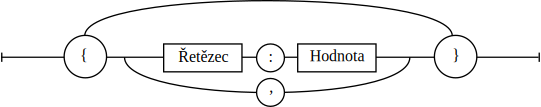
\includegraphics[width=0.8\textwidth]{jsonObject}
\caption{JSON Objekt}
\label{fig:jsonObject}
\end{figure}

\begin{figure}[htb]
\centering
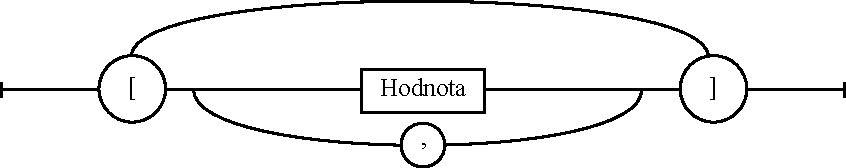
\includegraphics[width=0.8\textwidth]{jsonArray}
\caption{JSON Pole}
\label{fig:jsonArray}
\end{figure}

\begin{figure}[htb]
\centering
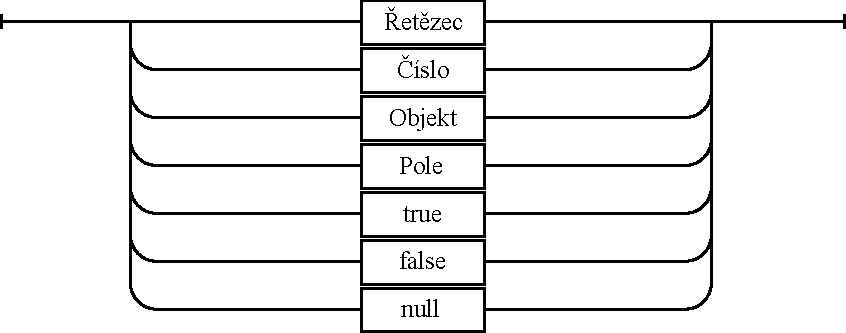
\includegraphics[width=0.8\textwidth]{jsonValue}
\caption{JSON Hodnota}
\label{fig:jsonValue}
\end{figure}

JSON je ve hře použit pro reprezentaci herních úrovní. Vzhledem k tomu, že při použití jakéhokoliv jiného formátu by bylo potřeba na vstupu provádět jeho parsování, což by hru zbytečně zpomalovalo, je tento formát v podstatě jediným vhodným kandidátem.

\section{Lineární algebra pro 3D grafiku}
\label{section:linearniAlgebra}
Lineární algebra je ta část matematiky, která se zabývá vektory a maticemi. Pro porozumění 3D grafice a WebGL je dobré mít alespoň základní znalosti v tomto oboru. Vzhledem k rozsahu této práce není možné zmínit vše, a proto jsou pojmy jako souřadný systém, vektory a jejich skalární a vektorový součin považovány za znalost čtenáře. Následující text se soustředí na homogenní souřadnice, matice a transformace ve 3D grafice.

\subsection*{Homogenní souřadnice}
\label{subsection:homogenniSouradnice}
V 3D prostoru je možné bod\footnote{Ve 3D grafice nazývaný \textit{vertex}} definovat pomocí tří souřadnic. To však může být matoucí v tom, že body a vektory jsou definovány stejným způsobem. S homogenními souřadnicemi přidáváme čtvrtou souřadnici, která je značena jako \textit{w}. Pro vektory je pak $w=0$, a pokud je $w!=0$, pak homogenní souřadnice definují bod. Homogenní bod lze převést na tříprvkový bod vydělením všech souřadnic souřadnicí homogenní. Pro převod tříprvkového bodu na bod homogenní pak stačí přidat jako homogenní souřadnici hodnotu 1. Homogenní souřadnice se používají z toho důvodu, že ve 3D grafice jsou nejčastější operací různé transformace, které jsou popsány pomocí $4\times4$ matic. Abychom mohli bod pomocí těchto matic transformovat, je nutné, aby byl bod popsán právě čtyřmi souřadnicemi.

\subsection*{Matice}
\label{subsection:matice}
Matice je složena z řádků a sloupců. Elementy uvnitř matice se nazývají prvky matice a dle počtu řádků a sloupců rozlišujeme různé její dimenze. Nejčastěji používaným typem jsou ve WebGL matice se čtyřmi řádky a čtyřmi sloupci. Tyto pak označujeme jako $4\times4$ matice.

\begin{equation}
 M = \begin{bmatrix}
       m_{00} & m_{01} & m_{02} & m_{03}     \\[0.3em]
       m_{10} & m_{11} & m_{12} & m_{13}     \\[0.3em]
       m_{20} & m_{21} & m_{22} & m_{23}     \\[0.3em]
       m_{30} & m_{31} & m_{32} & m_{33}     \\[0.3em]
     \end{bmatrix}
\end{equation}

Maticím s jedním sloupcem ($m \times 1$) se také jinak říká sloupcový vektor a maticím s jedním řádkem řádkový vektor ($1 \times m$).

\begin{align}
%\begin{split}
 V = \begin{bmatrix}
       v_{0} \\[0.3em]
       v_{1} \\[0.3em]
       v_{2} \\[0.3em]
       v_{3} \\[0.3em]
     \end{bmatrix} \\
%\end{split}
%\begin{split}
V = \begin{bmatrix}
       v_{0} & v_{1} & v_{2} & v_{3}  \\[0.3em]
     \end{bmatrix}
%\end{split}\tag{2.2a, 2.2b} 
\end{align}
%\tag{1a,b} 

\myparagraph{Součet a rozdíl matic}
Součet a rozdíl je možný, pokud mají matice stejné dimenze. Součet, nebo rozdíl pak probíhá prvek po prvku.


\begin{align}
%\begin{split}
 A = \begin{bmatrix}
       1 & 5 & 3 \\[0.3em]
       4 & 4 & 1 \\[0.3em]
     \end{bmatrix} \\
%\end{split}
%\begin{split}
 B = \begin{bmatrix}
       5 & 3 & 3 \\[0.3em]
       2 & 5 & 2 \\[0.3em]
     \end{bmatrix} \\
%\end{split}\tag{2.3a, 2.3b} 
%\end{align}
%\begin{align}
 A + B = \begin{bmatrix}
       6 & 8 & 6 \\[0.3em]
       6 & 9 & 3 \\[0.3em]
     \end{bmatrix}
\end{align}

\myparagraph{Násobení matic}
Násobení matic je ve 3D grafice velmi důležitou operací. Definice násobení je taková, že dvě matice mohou být vzájemně vynásobeny pouze tehdy, když se počet sloupců první matice rovná počtu řádků matice druhé. Výsledná matice má pak počet řádků rovný matici první a počet sloupců matici druhé.

\begin{align}
[m \times p][p \times n] = [m \times n]
\end{align}

Prvky \textit{ij} výsledné matice vzniknou skalárním vynásobením řádku \textit{i} matice \textbf{A} a sloupce \textit{j} matice \textbf{B}.

\begin{align}
M = 
\begin{bmatrix*}[r]
  -3 & 1 \\
  -2 & 2 \\
  -4 & 5 \\
\end{bmatrix*} \\
N =
\begin{bmatrix*}[r]
  -4 & 3 \\
   3 & 5 \\
\end{bmatrix*}
\end{align} 
\begin{align}
M \times N = 
\begin{bmatrix*}[r]
  (-3) \times (-4) + 1 \times 3 & (-3) \times 3 + 1 \times 5 \\
  (-2) \times (-4) + 2 \times 3 & (-2) \times 3 + 2 \times 5 \\
  (-4) \times (-4) + 5 \times 3 & (-4) \times 3 + 5 \times 5 \\
\end{bmatrix*}
=
\begin{bmatrix*}[r]
  15 & -4 \\
  14 & 4 \\
  31 & 13 \\
\end{bmatrix*}
\end{align}


\myparagraph{Matice identity a inverzní matice}
Matice identity je takovou maticí, že pokud s ní vynásobíme jakoukoliv matici jinou, tak získáme opět tu samou.

\begin{align}
M \times I = I \times M = M
\end{align}

Matice identity je vždy čtvercová (stejný počet sloupců jako řádků), na své diagonále má prvky rovny 1 a mimo diagonálu 0.

\begin{align}
I = 
\begin{bmatrix*}[r]
  1 & 0 & 0 & 0 \\
  0 & 1 & 0 & 0 \\
  0 & 0 & 1 & 0 \\
  0 & 0 & 0 & 1 \\
\end{bmatrix*}
\end{align}

Nyní, když víme, co je to matice identity, můžeme přistoupit k definici matice inverzní. Pro jakékoliv číslo $x$ (kromě 0) nalezneme číslo $1/x$ (zapisováno také jako $x^{-1}$), které při vynásobení touto inverzní hodnotou dává jako svůj výsledek hodnotu 1. Podobně je definována i matice inverzní, kterou označujeme jako $M^{-1}$.

\begin{align}
M \times M^{-1} = M^{-1} \times M = 1
\end{align}

Je důležité poznamenat, že pouze čtvercové matice mají matici inverzní.

\myparagraph{Transponovaná matice}
Transponovaná matice vznikne prohozením svých řádků se sloupci. Matice je definována pro jakékoliv dimenze a označuje se jako $M^{T}$. Vzhledem k tomu, že ve WebGL se používají matice $4\times4$, jsou i zde příklady uvedeny v těchto dimenzích.

\begin{align}
 M = 
\begin{bmatrix*}[r]
  1 & 2 & 3 & 4 \\
  5 & 6 & 7 & 8 \\
  9 & 10 & 11 & 12 \\
  13 & 14 & 15 & 16 \\
\end{bmatrix*}
\end{align}

\begin{align} 
M^T = 
\begin{bmatrix*}[r]
  1 & 5 & 9 & 13 \\
  2 & 6 & 10 & 14 \\
  3 & 7 & 11 & 15 \\
  4 & 8 & 12 & 16 \\
\end{bmatrix*}
\end{align}

\subsection*{Transformace}
\label{subsection:transformace}
Transformace je operace, která na svém vstupu přijímá jakousi entitu, jakou je například bod, nebo vektor, a nějakým způsobem ji modifikuje. Speciálním typem transformace je pak transformace lineární, což je zobrazení $f$ z jednoho vektorového prostoru do druhého $f: V \rightarrow W$, které zachovává vektorové operace sčítání a násobení skalárem. Název \textit{lineární} je odvozen z faktu, že grafem obecného lineárního zobrazení z reálných čísel do reálných čísel je přímka.

Mějme dva vektory $u$, $v$ a transformaci reprezentovanou pomocí funkce $f$. Pak lineární transformací je operace, která splňuje následující podmínky:

\begin{align}
\begin{split}
f(u) + f(v) = f(u+v) 
\end{split}
\begin{split}
 (aditivita)
\end{split} \\
\begin{split}
kf(u) = f(ku)
\end{split}
\begin{split}
 (homogenita)
 \end{split}
\end{align}


Mezi lineární transformace patří například posunutí (translace), rotace, změna měřítka (scaling), či zkosení (shearing). Násobením transformačních matic lze vytvářet ze základních transformací transformace komplexní. Při násobení však musíme dávat pozor na pořadí, ve kterém jsou matice násobeny. Násobení matic totiž není komutativní operací. Jakákoliv transformace bodu, nebo vektoru v 3D prostoru může být vyjádřena pomocí $4 \times 4$ matice.

\begin{align} 
Mv = \begin{bmatrix*}[r]
  m_{00} & m_{01} & m_{02} & m_{03} \\
  m_{10} & m_{11} & m_{12} & m_{13} \\
  m_{20} & m_{21} & m_{22} & m_{23} \\
  m_{30} & m_{31} & m_{32} & m_{33} \\
\end{bmatrix*}
\begin{bmatrix*}[r]
 v_{0} \\
 v_{1} \\
 v_{2} \\
 v_{3} \\
\end{bmatrix*} =
\begin{bmatrix*}[r]
  m_{00}v_{0} & m_{01}v_{1} & m_{02}v_{2} & m_{03}v_{3} \\
  m_{10}v_{0} & m_{11}v_{1} & m_{12}v_{2} & m_{13}v_{3} \\
  m_{20}v_{0} & m_{21}v_{1} & m_{22}v_{2} & m_{23}v_{3} \\
  m_{30}v_{0} & m_{31}v_{1} & m_{32}v_{2} & m_{33}v_{3} \\
\end{bmatrix*}
\end{align}

\pagebreak
\myparagraph{Translace}
Translace je lineární transformací, která posouvá bod v prostoru. Translační matice vypadá následovně:

\begin{align}
T(t_x, t_y, t_z) = 
\begin{bmatrix*}[r]
 1 & 0 & 0 & t_x \\
 0 & 1 & 0 & t_y \\
 0 & 0 & 1 & t_z \\
 0 & 0 & 0 & 1 \\
\end{bmatrix*}
\end{align}

Uvedená translační matice posouvá bod s ofsetem, který je reprezentován pomocí vektoru $(t_x, t_y, t_z)$. Diagram~\ref{fig:translation} znázorňuje translaci bodů krychle násobením s následující maticí:

\begin{align}
T(4, 5, 0) = 
\begin{bmatrix*}
1 & 0 & 0 & 5 \\
0 & 1 & 0 & 0 \\
0 & 0 & 1 & 0 \\
0 & 0 & 0 & 1 \\
\end{bmatrix*}
\end{align}

\begin{figure}[htb]
\centering
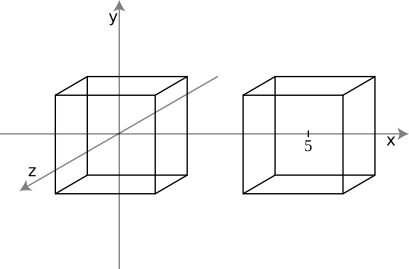
\includegraphics[width=0.8\textwidth]{translation}
\caption{Translace}
\label{fig:translation}
\end{figure}


\subsection*{Rotace}
Tato transformace rotuje bod, či vektor o zadaný úhel kolem počátku souřadného systému $[0, 0, 0]$. Běžně se používají rotační matice pro rotaci kolem osy\footnote{Rotace se řídí tzv. pravidlem pravé ruky. Palec směřuje v kladném směru osy a zbylé zatočené prsty ruky naznačují směr kladné rotace.} x, y a z. 

\begin{align}
R_x(\phi) = 
\begin{bmatrix*}
1 & 0 & 0 & 0 \\
0 & \cos\phi & -\sin\phi & 0 \\
0 & \sin\phi & \cos\phi & 0 \\
0 & 0 & 0 & 1 \\
\end{bmatrix*}
\end{align}

\begin{align}
R_y(\phi) = 
\begin{bmatrix*}
\cos\phi & 0 & \sin\phi & 0 \\
0 & 1 & 0 & 0 \\
-\sin\phi & 0 & \cos\phi & 0 \\
0 & 0 & 0 & 1 \\
\end{bmatrix*}
\end{align}

\begin{align}
R_z(\phi) = 
\begin{bmatrix*}
\cos\phi & -\sin\phi & 0 & 0 \\
\sin\phi & \cos\phi & 0 & 0 \\
0 & 0 & 1 & 0 \\
0 & 0 & 0 & 1 \\
\end{bmatrix*}
\end{align}

Diagram~\ref{fig:rotation} znázorňuje rotaci bodů krychle kolem počátku soustavy souřadnic s využitím této transformační matice:

\begin{align}
R_x(30^{\circ}) = 
\begin{bmatrix*}
1 & 0 & 0 & 0 \\
0 & \cos(30^{\circ}) & -\sin(30^{\circ}) & 0 \\
0 & \sin(30^{\circ}) & \cos(30^{\circ}) & 0 \\
0 & 0 & 0 & 1 \\
\end{bmatrix*}
\end{align}

\begin{figure}[htb]
\centering
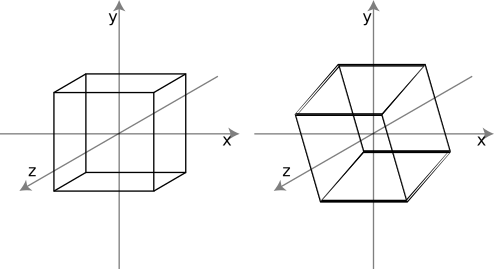
\includegraphics[width=0.8\textwidth]{rotation}
\caption{Rotace}
\label{fig:rotation}
\end{figure}

Dalšími transformacemi používanými ve 3D grafice je tzv. scaling, který zvětšuje, či zmenšuje objekt a pak tzv. shearing, který dokáže objekt zkosit dle dané osy. Tyto dvě transformace však nejsou při implementaci hry využity, a tudíž zde nebudou zmíněny.

\pagebreak
\section{WebGL}
\label{section:webgl}
WebGL je nízkoúrovňové aplikační rozhraní pro zobrazení pokročilé 3D grafiky na webu. Je založeno na OpenGL ES 2.0 a umožňuje programátorovi použít hardwarově akcelerované\footnote{K hardwarové akceleraci je nutno vlastnit GPU s podporou minimálně shader modelu 2.0. V opačném případě lze obraz vykreslovat softwarově.} vykreslování obrazu v kontextu HTML a JavaScriptu. Vykreslovací plochou, která je zde použita je HTML5 \texttt{<canvas>} element a jeho \texttt{webgl}, resp. \texttt{experimental-webgl} kontext.~\cite{seidelin2011html5}

\subsection*{Historie WebGL}
\label{subsection:historieWebGL}
První experimenty s 3D grafikou v \texttt{<canvas>} elementu prováděl Vladimir Vukićević ze společnosti Mozilla. Výsledkem jeho pokusů se stal prototyp, který nazval Canvas 3D. V roce 2009 vytvořila Khronos Group novou pracovní skupinu pro WebGL, která byla složena z hlavních tvůrců webových prohlížečů včetně firem jako Apple, Google, Mozilla a Opera. Khronos Group je neziskovou organizací, která vytváří a spravuje otevřené standardy a aplikační rozhraní. Byla založena roku 2000 a mimo jiné stojí i za standardy jako OpenGL, či výše zmíněným OpenGL ES, které je primárně určeno pro vestavěné systémy.~\cite{anyuru2012professional}

Finální specifikace WebGL 1.0\footnote{\url{http://www.khronos.org/registry/webgl/specs/1.0/}} byla vydána v březnu roku 2011 a její implementaci můžeme nalézt v prohlížečích jako Google Chrome, Mozilla Firefox, Safari a v počátečních fázích implementace v prohlížeči Opera. V případě Microsoft Internet Exploreru je situace poněkud odlišná. Microsoft neohlásil žádný záměr v podpoře WebGL ve svém prohlížeči. Uživatelé, kteří chtějí WebGL používat, jsou tedy nuceni přejít k jinému prohlížeči.~\cite{anyuru2012professional}

\subsection*{Výhody WebGL}
\label{subsection:vyhodyWebGL}
V dobách, kdy web jako takový začínal, byl jeho obsah vytvořen ze statických dokumentů. Hlavní prací webových prohlížečů tehdy bylo takovýto obsah získat a zobrazit. V průběhu času však webové technologie značně pokročily a nyní tak jejich prostřednictvím mužeme přistupovat k plnohodnotným webovým aplikacím s bohatým uživatelským rozhraním a audiovizuálním obsahem. Tyto aplikace se nyní stávají alternativou k aplikacím nativním.~\cite{anyuru2012professional} \\ \\
Jejich hlavními výhodami jsou:
\begin{itemize}
\item Rychlá \textbf{dostupnost} a jednoduchá \textbf{distribuce} mezi mnoho uživatelů.
\item \textbf{Snadná údržba a aktualizace aplikací.} Pokud je v aplikaci nalezena chyba, nebo pokud chceme rozšířit její funkcionalitu, pak vše, co je potřeba, je aktualizovat aplikaci na serveru a uživatelé mají ihned přístup k její nové verzi.
\item \textbf{Multiplatformnost aplikací.} Vše, co uživatel potřebuje je kompatibilní webový prohlížeč schopný zobrazit námi definovaný obsah.
\end{itemize}

Oproti nativním aplikacím nejsou ty webové obsahem tak bohaté, avšak s příchodem HTML5 začíná tento rozdíl mizet. Prostřednictvím WebGL je nyní možné zobrazovat hardwarově akcelerovanou grafiku přímo uvnitř prohlížeče. Je tak možné vytvořit 3D hry, nebo pokročilé 3D grafické aplikace a zároveň těžit z výhod webu, jak byli popsány výše. Technologie WebGL má navíc i další výhody, mezi něž patří například:
\begin{itemize}
\item WebGL je otevřený standard, který může používat každý bez poplatků.
\item WebGL využívá přímo grafický hardware, což znamená, že jsou aplikace rychlé.
\item Vzhledem k tomu, že je WebGL založeno na OpenGL ES, je možné vytvořené aplikace spouštět i na mnohých moderních mobilních zařízeních.
\end{itemize}

\subsubsection*{Grafická API}
\label{subsection:grafickaAPI}
Existují dva fundamentální přístupy, které jsou u grafických aplikačních rozhraní využity. Jsou jimi:
\begin{itemize}
\item immediate-mode API a 
\item retained-mode API,
\end{itemize}
přičemž WebGL používá první ze zmíněných přístupů.


\myparagraph{Immediate-mode API} 
U tohoto typu rozhraní je celá scéna překreslena s každým snímkem bez ohledu na to, zda byla změněna, či nikoliv. Grafická knihovna která zprostředkovává rozhraní programátorovi neukládá žádnou interní reprezentaci scény, která má být vykreslena. Reprezentaci scény je tak nutné uchovávat v paměti vlastní aplikace. Tento přístup je vysoce flexibilní a poskytuje programátorovi větší úroveň kontroly nad výsledným vykreslovaným obrazem. Na druhou stranu však tento přístup vyžaduje ze strany programátora více úsilí oproti přístupu, který si popíšeme nyní.

\begin{figure}[htb]
\centering
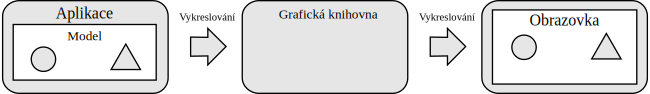
\includegraphics[width=0.8\textwidth]{immediateMode}
\caption{Immediate-mode API}
\label{fig:immediateMode}
\end{figure}

\myparagraph{Retained-mode API} 
U tohoto přístupu je interní model a veškeré vykreslované objekty scény obsažen v grafické knihovně, která toto rozhraní programátorovi nabízí. Programátor využívá přístupových metod k rozhraní a knihovna sama rozhoduje o tom, zda má být scéna a s ní její interní reprezentace aktualizována, či nikoliv. To znamená, že aplikace, která rozhraní využívá, nemusí v každém vykreslovaném snímku scénu překreslovat. Tento přístup je v mnohých ohledech pro programátora méně náročný a používá se například pro vykreslování vektorové grafiky (SVG). 

\begin{figure}[htb]
\centering
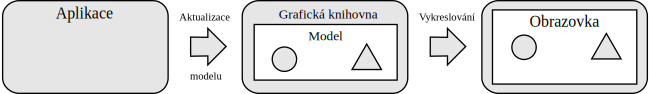
\includegraphics[width=0.8\textwidth]{retainedMode}
\caption{Retained-mode API}
\label{fig:retainedMode}
\end{figure}
 
\subsection*{Tvorba obrazu v grafickém hardwaru}
\label{subsection:tvorbaObrazu}
WebGL je nízkoúrovňové rozhraní a pracuje tak velmi blízko grafického hardwaru. K pochopení fundamentálních konceptů použitých při implementaci hry je tedy nejprve potřeba alespoň okrajově osvětlit, jakým způsobem grafický hardware pracuje. 

Na diagramu~\ref{fig:gpuDisplay} je zjednodušeně znázorněn vztah grafického hardwaru k ostatním částem systému.

\begin{figure}[htb]
\centering
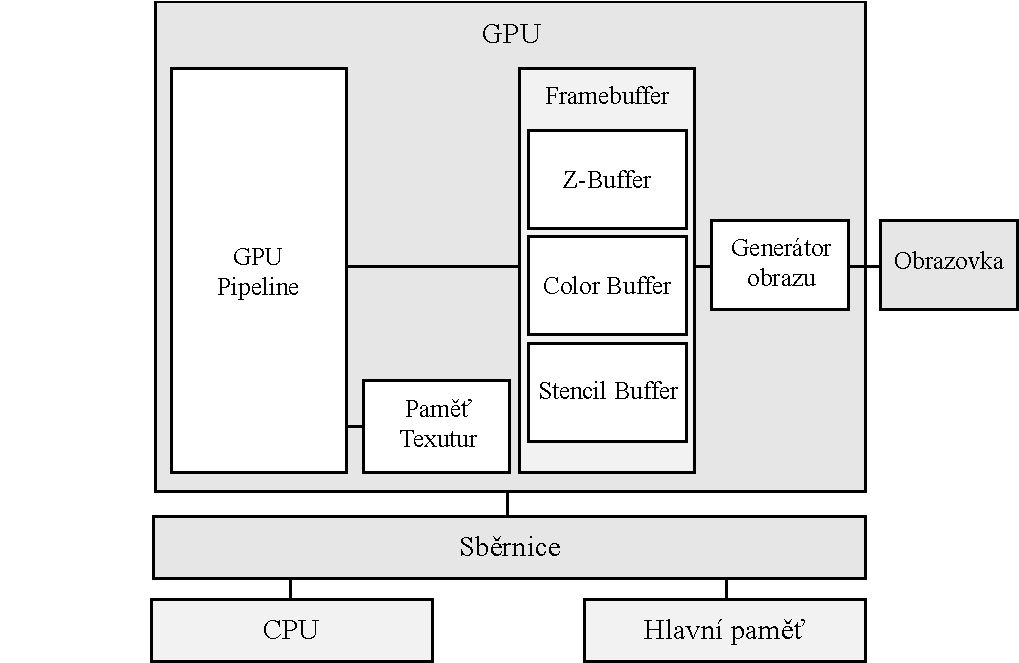
\includegraphics[width=0.8\textwidth]{gpuDisplay}
\caption{Vztah grafického hardwaru k ostatním částem systému}
\label{fig:gpuDisplay}
\end{figure}

\myparagraph{GPU}
GPU, neboli také Graphics Processing Unit, je dedikované zařízení, které je přímo navrženo pro zobrazení grafiky. Architektura GPU je vysoce paralelizovaná a provádí operace s grafickými daty velmi rychle. Zpracování dat probíhá typicky zřetězeně v několika úrovních.

\myparagraph{Framebuffer}
Framebuffer je místem, kde je uložen výsledek operací provedených na GPU. Je to paměť, která obsahuje informace nutné pro zobrazení výsledného obrazu na zobrazovací zařízení. V jednoduchém grafickém systému může být fyzická paměť framebufferu součástí hlavní operační paměti, avšak u moderních systémů je tato paměť alokována ve speciální rychlé grafické paměti na GPU. Framebuffer se typicky skládá ze tří odlišných \textit{subbufferů}.

\begin{itemize}
\item Color Buffer
\item Z-Buffer
\item Stencil Buffer
\end{itemize}

\mysubparagraph{Color Buffer}
Color buffer představuje dvourozměrné pole, jehož prvky jsou výsledné barvy pixelů obrazu. Každý z těchto prvků obsahuje informaci o výsledné barvě v RGB, či RGBA formátu. Každý z barevných kanálů má alokován určitý počet bitů a navíc může být obsažena informace o \textit{alpha} kanálu, který určuje viditelnost daného pixelu. Celkový počet bitů použitých pro jeden pixel je označován jako barevná hloubka (color depth). \\ \\ Varianty barevné hloubky:

\begin{itemize}
\item 16 bitů na pixel
\item 24 bitů na pixel
\item 32 bitů na pixel
\end{itemize} 

Barevná hloubka 16 bitů se často používá na menších zařízeních. Je zde použito systému RGB565, který zohledňuje zvýšenou citlivost lidského oka na zelenou barvu. Rozložení jednotlivých barevných kanálů tedy není rovnoměrné a je alokováno 5 bitů pro červenou barvu, 6 bitů pro barvu zelenou a 5 bitů pro barvu modrou. Barevná hloubka 24 bitů má pak pro každou barvu alokováno po osmi bitech a v případě barevné hloubky 32 bitů je dalších 8 bitů alokováno pro alpha kanál.

\mysubparagraph{Z-Buffer}
Jak již bylo uvedeno v předchozím odstavci, color buffer typicky obsahuje barvy pixelů výsledného obrazu. V zobrazované scéně jsou však některé vykreslované objekty překryty jinými a pixely, které těmto zakrytým objektům náleží, by tak neměly být viditelné. Toho je docíleno pomocí z-bufferu, který má stejný počet prvků jako color buffer, avšak není zde uložena barva, nýbrž vzdálenost pozorovatele od nejbližšího objektu scény. Ta následně rozhoduje o tom, jaký objekt má být v daném pixelu vykreslen a který nikoliv. V souvislosti s implementací je tento buffer využíván pouze v případě, že objekty scény nejsou zprůhledněny.

\mysubparagraph{Stencil Buffer}
Jako doplněk ke dříve popsaným bufferům je na moderním grafickém hardwaru přítomen i stencil buffer, který určuje to, kam má být aktuálně zpracovávaný objekt scény vykreslen v rámci color bufferu. V praxi je tento buffer využit například pro vykreslování stínů. Stíny nejsou v implementaci použity, proto se již dále stencil bufferem nebudeme zabývat.

\subsection*{Grafická pipeline}
\label{subsection:pipeline}
Webové aplikace jsou typicky složeny z HTML, CSS a JavaScriptových souborů, které jsou interpretovány a zobrazovány prohlížečem. Aplikace využívající WebGL navíc obsahuje zdrojový kód shaderů a data, která reprezentují 3D scénu. JavaScript využívá rozhraní WebGL, aby předal této knihovně zdrojové kódy programovatelných součástí grafické pipeline a data, která reprezentují vykreslovaný 3D model. Poté, co jsou data knihovně předána, je výsledek vykreslen do tzv. \textit{drawing bufferu}, což je ve své podstatě framebuffer pro WebGL. Stejně tak jako framebuffer obsahuje color, stencil a z-buffer, avšak jeho obsah je nejdříve spojen se zbytkem webové stránky a teprve poté končí ve framebufferu fyzickém. V implementaci hry je využito 32 bitové varianty drawing bufferu a je tak tedy možné využít alpha kanálu na prolínání vykreslované 3D grafiky se svým okolím, resp. se zbytkem webové stránky. Grafická pipeline je zobrazena na diagramu~\ref{fig:gpuPipeline}.

\begin{figure}[htb]
\centering
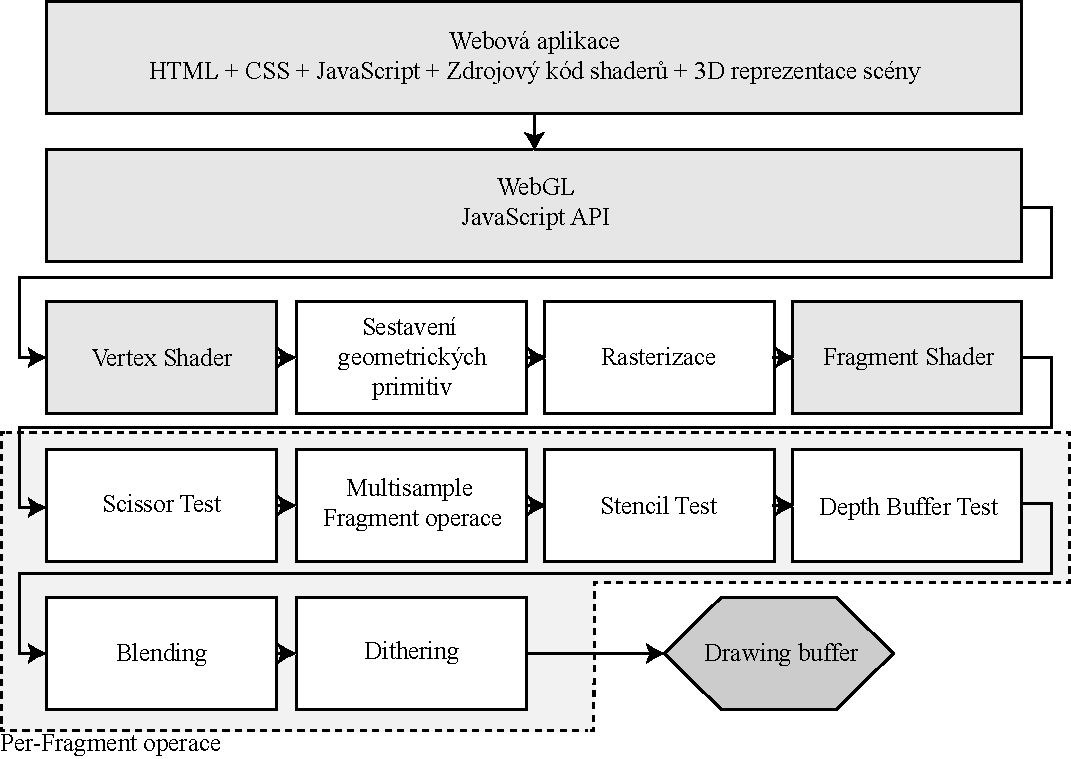
\includegraphics[width=0.8\textwidth]{gpuPipeline}
\caption{GPU pipeline}
\label{fig:gpuPipeline}
\end{figure}

K tomu, abychom získali realistickou 3D scénu nestačí pouze vykreslit objekty na určité pozice. Musíme také vzít v úvahu, jak budou objekty vypadat, pokud na ně bude dopadat světlo ze světelných zdrojů scény. Obecně se technice, která se používá ve spojitosti s působením světla na různé typy materiálů říká~\textit{shading}. Ve WebGL je shading rozdělen do dvou částí, jejichž chování je možné naprogramovat. \\ \\ Programovatelnými součástmi grafické pipeline jsou:
\begin{itemize}
\item Vertex Shader
\item Fragment Shader
\end{itemize}

\myparagraph{Vertex Shader}
První částí grafické pipeline, do které vstupují data předaná WebGL knihovně, je vertex shader. Jak již jeho název napovídá, provádí shading jednotlivých vertexů vykreslované scény. Než však samotný proces shadingu započne, je nutno vertexy transformovat a umístit tak objekt, jemuž vertexy náleží, na požadovanou pozici. Toho je docíleno pomocí transformačních matic, které jsou popsány v podkapitole~\ref{section:linearniAlgebra}. Vertex shader používá následující vstupy:
\begin{itemize}
\item Zdrojový kód vertex shaderu, který je zapsán v OpenGL ES Shading Language (GLSL ES).
\item Atributy, které definují data specifická každému vertexu. Typicky je to jeho pozice, normála a barva.
\item Tzv. \textit{uniform} proměnné, které jsou pro všechny vertexy objektu konstantní a lze je změnit až po dokončení operace vykreslování. Jedná se o transformační matice a dále pak například o pozice, na kterých se nachází světelné zdroje.
\end{itemize}

\begin{figure}[htb]
\centering
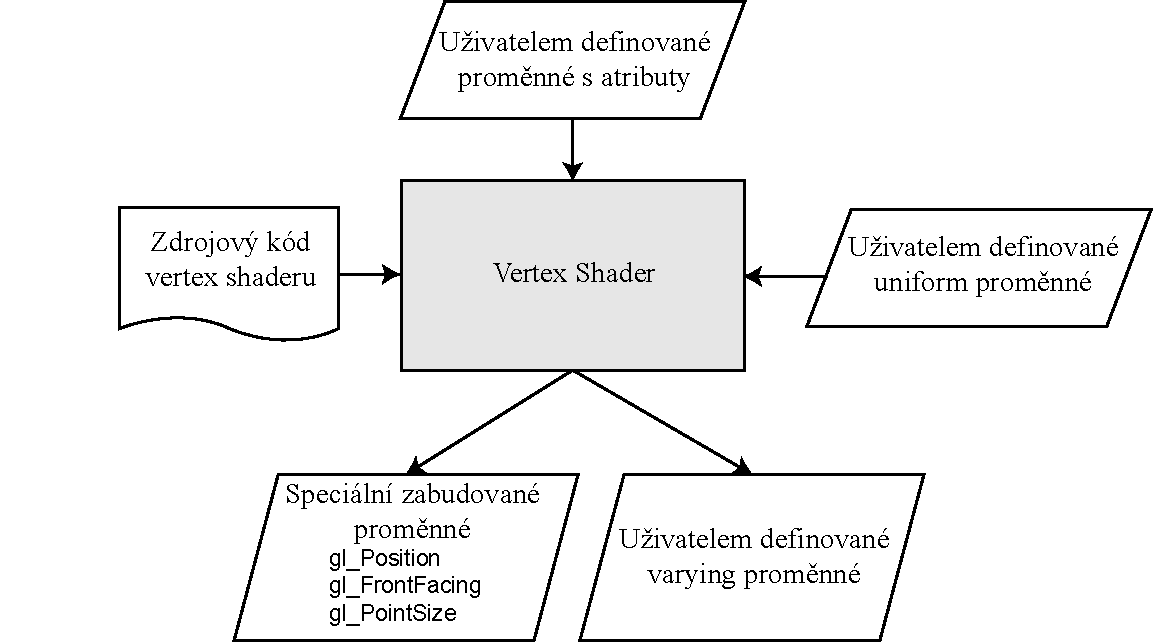
\includegraphics[width=0.8\textwidth]{vertexShader}
\caption{Vertex Shader}
\label{fig:vertexShader}
\end{figure}

Na diagramu~\ref{fig:vertexShader} jsou pak jestě znázorněny zabudované a uživatelky definované \textit{varying} proměnné. Využití varying proměnných je v delegaci informací z vertex shaderu do fragment shaderu. Jednou z nejdůležitějších speciálních zabudovaných proměnných je \texttt{gl\_Position}, která po práci vertex shaderu udává pozici, na které se vertex nachází. Popis vertex shaderu probíhá pomocí jazyka GLSL, který je svou syntaxí podobný programovacímu jazyku C. Příklad takového popisu je uveden ve zdrojovém kódu~\ref{code:vertexShader}

\begin{lstlisting}[caption=Ukázka zdrojového kódu GLSL pro vertex shader,label=code:vertexShader]
// Deklarace atributů vertexu
// Vektor pozice vertexu (XYZ)
attribute vec3 aVertexPos;
// Barva vertexu (RGBA)
attribute vec4 aVertexColor;

// Uniform proměnné
// Model-View Matice (4x4)
uniform mat4 uMVMatrix;
// Projekční matice (4x4)
uniform mat4 uPMatrix;

// Deklarace varying proměnné obsahující výstupní barvu vertexu, 
// která je vstupem pro fragment shader.
varying vec4 vColor;

void main() {
	// Transformace vertexu projekční a model-view maticí, kde
	// gl_Position udává jeho výslednou pozici ve scéně.
	gl_Position = UPMatrix * uMVMatrix * vec4(aVertexPos, 1.0);
	
	// Barva vertexu je poslána dále do fragment shaderu	.
	vColor = aVertexColor;
}
\end{lstlisting}
\pagebreak
\myparagraph{Sestavení primitiv}
V tomto kroku jsou sestaveny jednotlivé vertexy, které prošly skrze vertex shader, do geometrických primitiv, jakými jsou například trojúhelníky či hrany. Následně je potřeba rozhodnout o tom, zda je sestavený objekt v regionu, který je aktuálně viditelný na obrazovce. Tento region je označován jako \textit{frustrum} a je představován komolým jehlanem s obdélníkovou, či čtvercovou podstavou. Objekt který je uvnitř frustra je předán ke zpracování dalším částem grafické pipeline. Objekty, které jsou kompletně mimo frustrum, se odstraní, a ty, které jsou vně pouze částečně, budou oříznuty. Frustrum je znázorněno na diagramu~\ref{fig:frustrum}

\begin{figure}[htb]
\centering
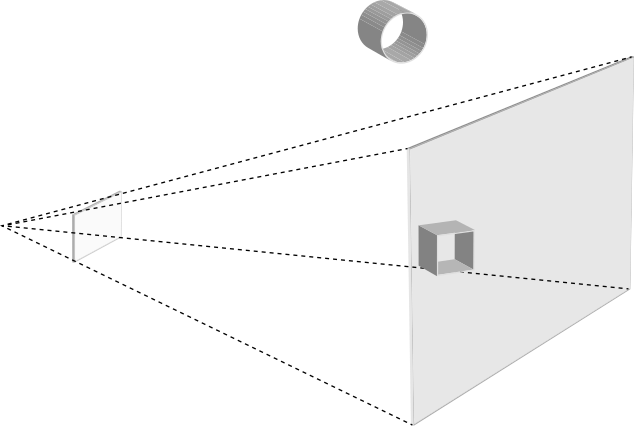
\includegraphics[width=0.8\textwidth]{frustrum}
\caption{Frustrum}
\label{fig:frustrum}
\end{figure}

\myparagraph{Rasterizace}
Dalším krokem je převod primitiv na fragmenty (diagram~\ref{fig:planeFragment}), pod kterými si můžeme představit jednotlivé pixely obrazovky. Fragmenty dále putují do fragment shaderu.

\begin{figure}[htb]
\centering
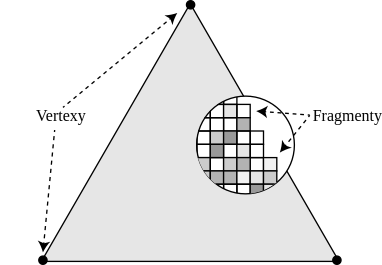
\includegraphics[width=0.8\textwidth]{planeFragment}
\caption{Fragmenty}
\label{fig:planeFragment}
\end{figure}

\myparagraph{Fragment shader}
Fragment shader je druhou programovatelnou součástí grafické pipeline. Jak již bylo zmíněno, fragment odpovídá pixelu, avšak ne všechny fragmenty se pixely stanou. Fragmenty totiž mohou být odstraněny v dalších částech pipeline. Fragment shader se svými vstupy a výstupy je znázorněn na diagramu~\ref{fig:fragmentShader}. Vstupem fragment shaderu jsou:
\begin{itemize}
\item Zdrojový kód fragment shaderu v jazyku OpenGL ES Shading Language.
\item Speciální zabudované proměnné, mezi něž patří například \texttt{gl\_PointCoord}.
\item Varying proměnné, které byli poslány skrze vertex shader.
\item Uniform proměnné, které obsahují konstanty společné všem fragmentům vykreslovaného objektu.
\item Samplery, což jsou speciální uniform proměnné určené pro texturování.
\end{itemize}

\begin{figure}[htb]
\centering
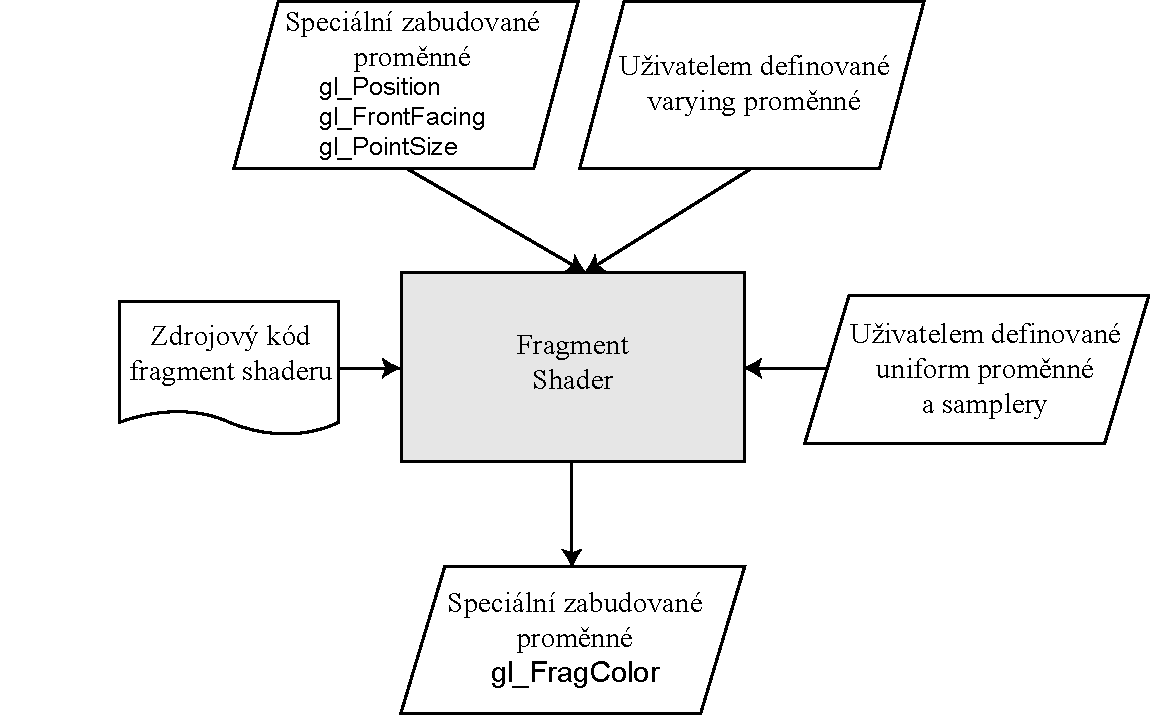
\includegraphics[width=0.8\textwidth]{fragmentShader}
\caption{Fragment Shader}
\label{fig:fragmentShader}
\end{figure}



Jak již bylo zmíněno dříve, varying proměnné slouží k posílání informací skrze vertex shader. Obecně však platí, že objekt má více fragmentů než vertexů. Obsah varying proměnných, který je zaslán skrze vertex shader, je lineárně interpolován pro každý fragment. 

Výsledek práce fragment shaderu je zapsán do zabudované proměnné \texttt{gl\_FragColor}, která následně obsahuje výslednou barvu daného fragmentu. Ve zdrojovém kódu~\ref{code:fragmentShader} je uveden příklad GLSL programu fragment shaderu, který pro každý fragment získá lineárně interpolovanou hodnotu s jeho barvou a uloží ji jako svůj výstup.

\label{code:fragmentShader}
\begin{lstlisting}[caption=Příklad jednoduchého GLSL programu fragment shaderu]
varying ver4 vColor;
void main(){
	gl_FragColor = vColor;
}
\end{lstlisting}

\myparagraph{Per-Fragment operace}
Každý fragment, který projde fragment shaderem, je postoupen do dalšího bloku pipeline, která se skládá z několika částí provádějící tzv. per-fragment operace. Každá z operací může ovlivnit výsledný pixel v drawing bufferu, avšak v implementaci je využito pouze blendingu a depth buffer testu. Zbylé části jsou uvedeny pro úplnost popisu pipeline.

\mysubparagraph{Scissor test}
Scissor test určuje, zda je zpracovávaný fragment uvnitř pravoúhlého rovnoběžníku, který je definován jedním bodem, výškou a šírkou. Fragmenty mimo tento rovnoběžník jsou zahozeny, ostatní pokračují dále v cestě grafickou pipeline.

\mysubparagraph{Multisample fragment operace}
Tato část pipeline modifikuje aplha kanál fragmentu, čímž je docíleno vyhlazení hran vykreslovaných objektů. Tato technika se obecně označuje jako \textit{anti-aliasing}.

\mysubparagraph{Stencil test}
Zde se fragment porovnává s nastavenou referenční hodnotou. Na základě výsledku porovnání je fragment opět zahozen, nebo postoupen dále.

\mysubparagraph{Depth buffer test}
Vzhledem k tomu, že se v téměř každé vykreslované scéně objekty překrývají, je nutné do color bufferu vykreslovat pouze ty objekty, které jsou viditelné. Tento test ve spolupráci s depth bufferem rozhoduje o tom, zda fragment vykreslovat, či nikoliv.

\mysubparagraph{Blending}
V dalším kroku označovaným jako blending jsou kombinovány barvy fragmentů, které jsou momentálně vykresleny do color bufferu na odpovídající pozici. Toho je v implementaci využito pro vykreslování průhledných objektů scény.

\mysubparagraph{Dithering}
Posledním krokem před vykreslením do color drawing bufferu je tzv. dithering. Vzhledem k tomu, že color buffer má omezený počet bitů k reprezentaci každé z barev, dithering tyto složí tak, že vytvoří iluzi toho, že máme k dispozici barev více.

%\subsection*{WebGL Frameworky}
%\label{subsection:webGLFrameworky}
%Specifikace neexistuje dlouhou dobu, avšak již dnes můžeme nalézt mnohé frameworky, které programování s WebGL značně usnadňují. Vzhledem k tomu, že použití WebGL frameworků nebylo při implementaci povoleno, má následující přehled pouze informativní charakter.

%Mezi nejznámější WebGL frameworky patří:
%\begin{itemize}
%\item C3DL
%\item Copperlicht
%\item GLGE
%\item SceneJS
%\item Three.js
%\item WebGLU
%\end{itemize}

%\subsection*{WebGL a bezpečnost}
%WebGL přistupuje přímo ke grafickému hardwaru, tudíž se mohou objevit situace, ve kterých je možné tuto skutečnost zneužít a vytvořit takový %WebGL dokument, který způsobí to, že grafická karta přestane reagovat na ostatní aplikace. Systémy Microsoft Windows tuto skutečnost detekují a %resetují grafickou kartu, avšak na systémech firmy Apple není tato detekce přítomna a takový dokument by potenciálně mohl zapříčinit pád %systému. U Linuxu záleží na verzi použitého ovladače grafické karty. Některé z nich blokaci detekují a některé nikoliv (například současný %ovladač grafických karet NVIDIA Nouveau). 

%\subsection*{Rychlost JavaScriptu v souvislosti s WebGL}
%Interprety JavaScriptu v prohlížečích se neustále vylepšují a dosahují tak vyšších rychlostí, avšak pro výpočetně složité operace je jeho %rychlost stále nízká. Pokud tedy chceme dosáhnout rychlého vykreslování, je potřeba přenechat co nejvíce práce grafickému hardwaru a jeho %shaderům. Na diagramu~\ref{webglPerformace} je uvedeno srovnání jednotlivých webových prohlížečů s  

%doplnit osvetlovaci modely a opacity


